\documentclass{article}

\pagestyle{empty}

\usepackage{csvsimple}
\usepackage{amsmath}
\usepackage{graphicx}
\usepackage{caption}
\usepackage[top=1cm, bottom=1cm, left=1cm, right=1cm]{geometry}

\begin{document}
	
	\begin{figure}[h]
    	\centering
    	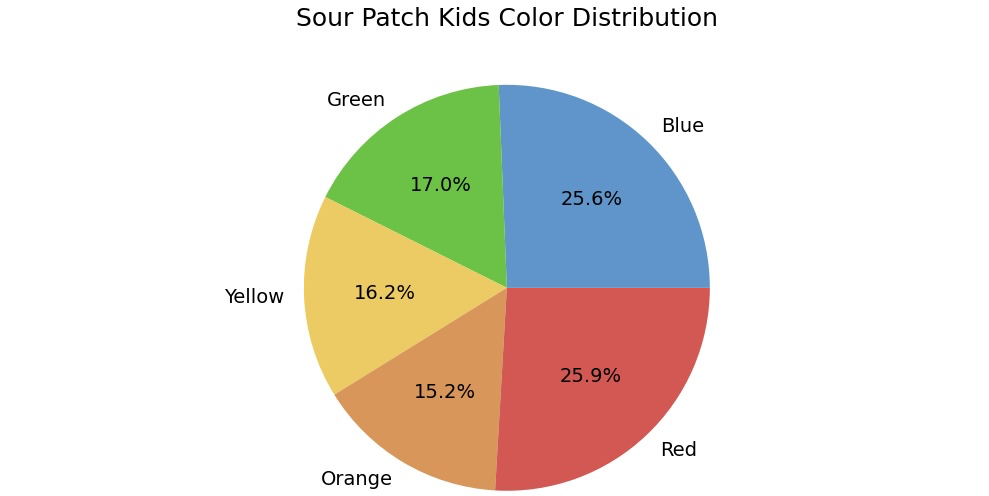
\includegraphics[width=1 \textwidth]{spkbarchart.png}
		\captionsetup{labelformat=empty}
    	\caption{}
    	\label{} 
	\end{figure}

	To prove that the distribution of Sour Patch Kids colors is not even 400 snack-sized packs were purchased, opened, and their colors recorded. With the resultant data a $X^{2}$ Test for Goodness of Fit can be conducted with the following hypotheses: 
	
	\begin{center}
		\begin{tabular}{l}
			$H_o$: The distribution of Sour Patch Kids colors is equal \\
			$H_A$: The distribution of Sour Patch Kids colors is not equal
		\end{tabular}

		\vspace{0.5cm}
		
		\begin{tabular}{|c|c|c|c|c|}
			\hline
			Color & Observed  & Expected & $O-E$ & $(O-E)^{2}$/E\\
			\hline
			\csvreader[late after line=\\]{spkstats.csv}{}{\csvcoli & \csvcolii & \csvcoliii & $\csvcoliv$ & $\csvcolv$}
			\hline
			Total & 2492 & & $X^{2}$ Statistic & 140.7889\\
			\cline{1-2} \cline{4-5}
		\end{tabular}
	\end{center}

	\vspace{0.25cm}

	\begin{minipage}[t]{0.4\textwidth}
		\vspace{0.475cm}
		The critical value can be found with the following: \vspace{0.3cm}
		
		\hspace{0.4cm}
		\begin{minipage}{\dimexpr\linewidth-0.5cm}
    		$df=4$ \\
    		$\alpha = 0.05$. \\
    		$X^{2}_{0.05,4}=9.02$ \\
    		$140.7889>9.02$; $X^{2}>X^{2}_{0.05,4}$
		\end{minipage}
		
		\vspace{0.5cm}
		\begin{center}
			$X^{2}>X^{2}_{0.05,4}$; Therefore \\
			there is sufficient evidence \\
			to reject $H_o$
		\end{center}

	\end{minipage}
	\hfill
	\begin{minipage}[t]{0.5\textwidth}
		\vspace{0cm}
		\centering
    	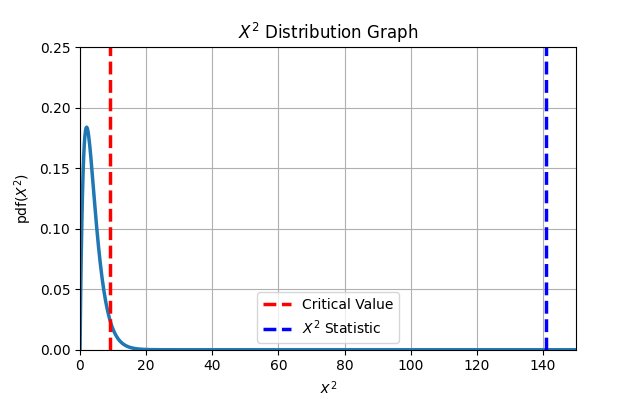
\includegraphics[width=1 \textwidth]{chisquaregraph.png}

		Any $X^{2}$ value to the right of the Critical Value would show there is significant evidence to reject the $H_{o}$
	\end{minipage}

	\vspace{0.25cm}

	With the results of the $X^{2}$ Test for Goodness of Fit, it is clear that there is significant evidence that the distribution of Sour Patch Kids is not equal. From the data of 400 packs and 2492 individual candies, it is clear there are a greater number of Red and Blue Sour Patch Kids than Green, Orange, and Yellow, with approximate distributions closer to $1/2$ Blue and Red, and $1/6$ Green, Orange, and Yellow.
\end{document}
